

%!TEX root = ./main.tex
\chapter{Of Server Sockets and their Characteristics 
\label{chapter:sockets}}

%%%%%%%%%%%%%%%%%%%%%%%%%%%%%%%%%%%%%%%%%%%%%%%%%%%%%%%%%%%%%%%%%%%%%%%%%%%%%%%%
% SERVER SOCKETS
%%%%%%%%%%%%%%%%%%%%%%%%%%%%%%%%%%%%%%%%%%%%%%%%%%%%%%%%%%%%%%%%%%%%%%%%%%%%%%%%
\section{Server Sockets} Since the Internet has moved from a research project to a widely used, public communication infrastructure, one of the critical success factors was its diversity with respect to network applications or services. This was heavily favored by the Internets layered design as described by the OSI model. 

Todays network applications ranges from traditional services as web, FTP or mail to new and emerging services as video streaming and social networks. However, the term network application or service is overloaded and are differently used depending on the actual technical context.

Since this thesis will operate with flow-level data, layer 5-8 in the OSI model are invisible in the data set. Therefore, network services can be differentiated only by information based on layer 3 and 4 of the OSI model of the two connection end-points. For this reason, the following abstractions of a connection end-point are defined:

%%%%%%%%%%% SOCKET DEFINITION 			%%%%%%%%%%%%%%%%%%%%%%
\parbox{ 
\textwidth}{ 
\begin{defn}
	{\textbf{Socket}\\} A socket is uniquely defined by the triple (\textbf{IP address}, \textbf{IP protocol number} and \textbf{protocol port number}). A socket is only defined for IP protocol TCP(6) and UDP(17). 
\end{defn}
}

%%%%%%%%%%% SERVER SOCKET DEFINITION 	%%%%%%%%%%%%%%%%%%%%%%
\parbox{ 
\textwidth}{ 
\begin{defn}
	{\textbf{Server Socket 
	\label{def:serversocket}}\\} A server socket is a socket with a process listening to incoming connections and thus offering a network service. The lifetime of a server socket is not restricted to individual connections, but by the lifetime of the network service. 
\end{defn}
}

%%%%%%%%%%% CLIENT SOCKET DEFINITION 	%%%%%%%%%%%%%%%%%%%%%%
\parbox{ 
\textwidth}{ 
\begin{defn}
	{\textbf{Client Socket}\\} A client socket is a socket which is only used to initiate a connection to a server socket. Therefore, client sockets are of temporary lifetime which is limited by the duration this connection. 
\end{defn}
}

In spite of the containment of the term \emph{server} in definition \ref{def:serversocket}, this definition is not only valid for server-client application protocols, but also holds for P2P-applications. 
\todo{Explain more?}


%%%%%%%%%%%%%%%%%%%%%%%%%%%%%%%%%%%%%%%%%%%%%%%%%%%%%%%%%%%%%%%%%%%%%%%%%%%%%%%%
% DETECTION OF SERVER SOCKETS
%%%%%%%%%%%%%%%%%%%%%%%%%%%%%%%%%%%%%%%%%%%%%%%%%%%%%%%%%%%%%%%%%%%%%%%%%%%%%%%%
\section{Detection of Server Sockets 
\label{section:socket_detection}}

% problem of detection with flow-level information (timing issue + flags)
Basically, a \emph{server socket} can be identified by the fact that a client opens a socket which initiates a connection to a \emph{server socket}. Usually, a \emph{client socket} is chosen at random by his operating system and the \emph{server socket} should be stable over time since it must offer a specific network service or application. Moreover, on each host a socket can only be assigned to one specific process per instance, i.e. a client socket connection initializing application or a \emph{server sockets} network application waiting on client connections. Otherwise, a socket-in-use-error is issued by the operating system. 

A straight-forward approach for detecting \emph{server sockets} is to infer the initiator of the connection by the timing information and determine its opposite as the \emph{server socket}. However, this approach requires a time synchronization of all flow exporting devices across the network. In practice, this can be hardly achieved in a satisfactory and reliable way.

% connection graph idea... +image
Hence, the detection of \emph{server sockets} with flow data relies on the following approach proposed by \citet{Schatzmann:Mining,Schatzmann:Dissection, Schatzmann:Tracing}. First of all, a communication graph is build as shown in figure \ref{fig:bipartite_graph}. This connection graph consists of nodes each representing an unique socket. If a bidirectional connection between two sockets is observed, an undirected, unweighted edge between the corresponding two nodes is assigned. This means that neither the direction nor the weight in terms of packets or bytes are required at all to build the connection graph. 
\begin{figure}
	[h] \centering 
	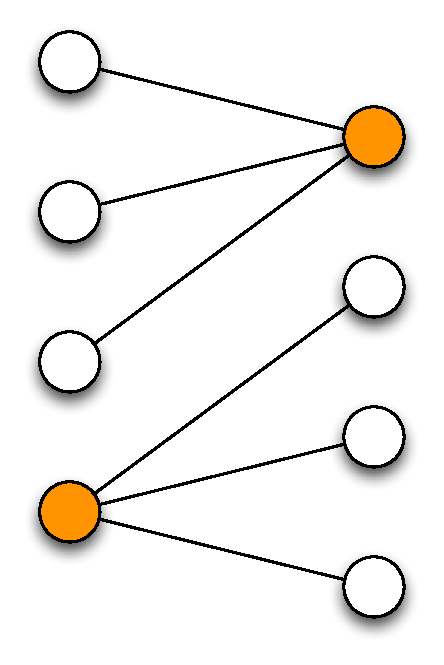
\includegraphics[width=\linewidth/3]{images/connection_graph.eps} \caption{Example of a bipartite connection graph with two concentrators of degree 3 marked as orange} 
	\label{fig:bipartite_graph} 
\end{figure}

In consequence of the fact that \emph{server sockets} provide a network application or service, they are likely to be contacted by several clients depending on their popularity. To this end, a socket which is contacted by a certain amount of client sockets and thus have a high degree in the connection graph is defined to be a \textbf{concentrator}. These concentrators are likely to offer a network service and are thus \emph{server sockets}. 
This approach is able to detect \emph{server sockets} which are offering not only classical client-server services,such as web, FTP, SSH, etc., but also p2p applications such as Skype, Bit-torrent super-nodes, etc. 
Therefore, it can be assumed that nodes with a high degree correspond to a \emph{server sockets}.

% introduce minimal vertex cover problem
\todo{Introduce Minimal vertex cover problem + recall + greedy algorithm}

% greedy algorithm to solve mvcp
% recalling sockets for optimization
\todo{Describe me!}
\begin{algorithm}[t!]
\caption{Detection of server sockets by \citet{Schatzmann:Mining,Schatzmann:Dissection, Schatzmann:Tracing}}
\label{alg:service_tracing_ss-detection}
\begin{algorithmic}
\STATE
\STATE compute list $SS_{in}$ \COMMENT{int. sockets sorted by \# ext. clients}
\STATE compute list $SS_{out}$ \COMMENT{ext. sockets sorted by \# int. clients}
\STATE
\WHILE{(deg($SS_{out}[0]$) $ > 2 $ \OR deg($SS_{in}[0]$)$ > 2$)}
    \WHILE {(deg($SS_{in}[0]$) $ > $ deg($SS_{out}[0]$))}
        \STATE $ss$ = $SS_{in}[0]$ \COMMENT{classify $ss$ as internal server socket}
        \STATE remove $ss$ from $SS_{in}$
        \STATE update deg() for all entries of $SS_{in}$
    \ENDWHILE
    \WHILE{(deg($SS_{out}[0]$) $ \geq $ deg($SS_{in}[0]$))}
        \STATE $ss$ = $SS_{out}[0]$ \COMMENT{classify $ss$ as external server socket}
        \STATE remove $ss$ from $SS_{out}$
        \STATE update deg() for all entries of $SS_{out}$
    \ENDWHILE
\ENDWHILE
\end{algorithmic}
\end{algorithm}

\begin{figure}
	[ht] \centering
	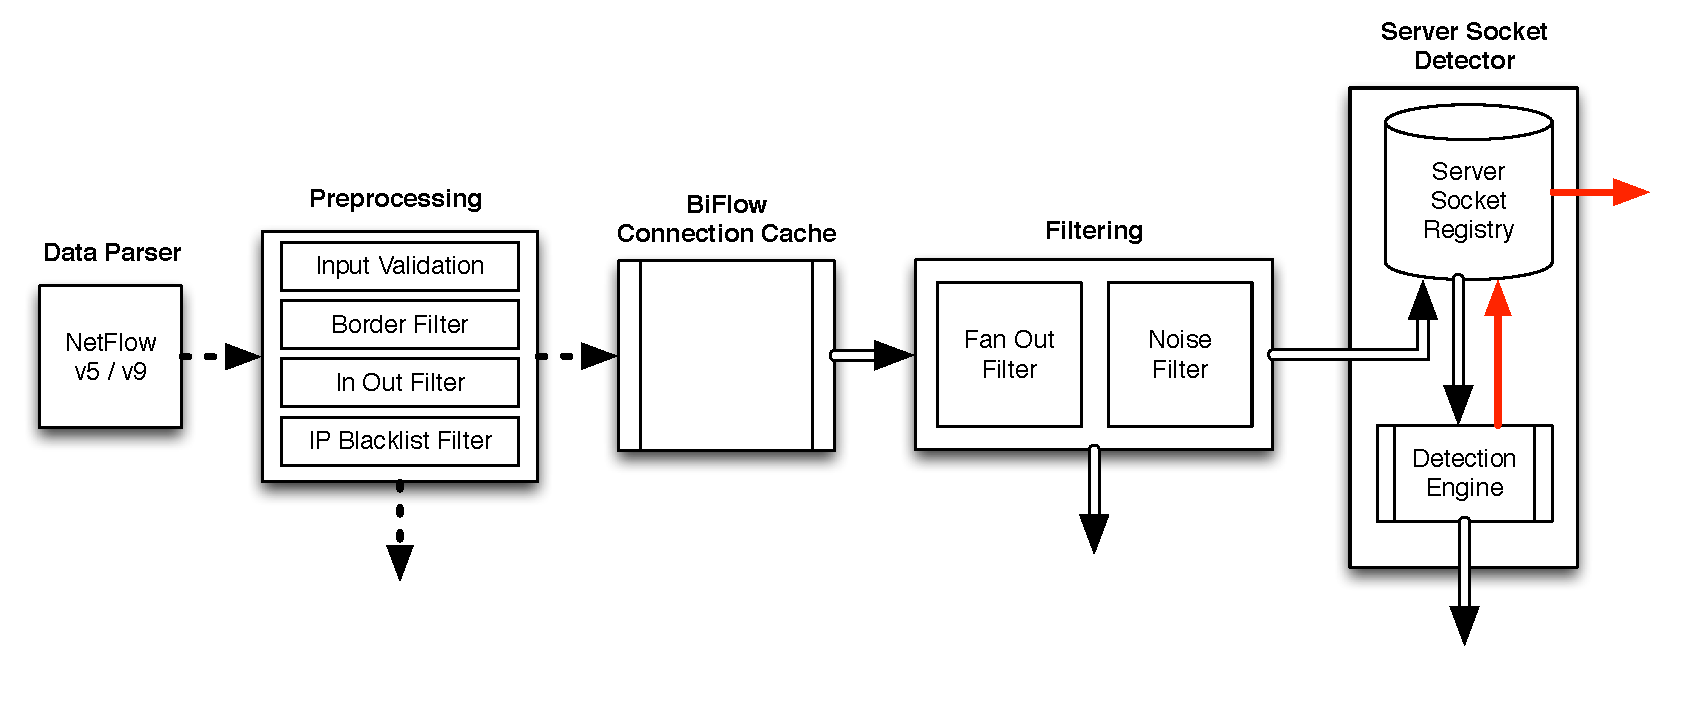
\includegraphics[width=\linewidth]{images/Detection_chain.eps}
	\caption{Processing chain for server socket detection} 
	\label{fig:detection_chain} 
\end{figure}

\subsection{Implementation}
Figure \ref{fig:detection_chain} illustrates the processing steps of the 
overall detection chain. The data parser is responsible to read the netflow data 
either in NetFlow v5 or NetFlow v9 format. These unidirectional flow records are 
then preprocessed by different blocks. While the input validator is performing 
some basic sanity checks of the flow data, the preprocessing filters are 
limiting the number of flows to the required kind of flow data. On the one hand, 
the border filter is removing all flow records not generated by a border router 
interface to efficiently prevent duplicate flow records. On the other hand, the 
In-Out filter is removing all non cross-border traffic, i.e. transit traffic 
(external to external) or entirely internal traffic (internal to internal). 
Furthermore, the IP blacklist filter is removing traffic towards blacklisted IP 
addresses or networks.

The connection cache is responsible for summarizing all related unidirectional 
flow records into a single bidirectional flow record during an aggregation 
period. After this caching step, these bidirectional flows are filtered by a fan 
out filter implementing the idea of \citet{Allman:2007} to mitigate the effects 
of scanning and p2p churn. This scanning detection filter is discussed in more 
detail by \citet{Schatzmann:Mining,Schatzmann:Dissection, Schatzmann:Tracing}. 

Afterwards, the remaining bidirectional flow records are again reduced by the 
noise filter. This last filtering module is responsible to filter bidirectional 
flow records which does not represent a correct bidirectional connection. A 
correct bidirectional connection is simply defined as either a correct TCP 
handshake or a reply flow as in case of UDP. Hence, the approach of deducing 
correct connections is to investigate the number of packets for each direction 
of the bidirectional flow record, i.e. the outgoing and the incoming flow 
record, since there are only cross-border flows remaining due to the In-Out 
filter. If a bidirectional TCP flow has in a single direction less than 3 
packets, the filter assumes that this flow does not represent a correct 
connection and is filtering this record. Accordingly, a bidirectional UDP 
flow is required to consist of at least 1 packet for each unidirectional flow 
record.

After these filtering steps, the remaining bidirectional flows are passed to the 
server socket detector which is finally performing the server socket detection 
approach previously discussed. Mainly, the server socket detector is build from 
two main parts. On the one side, there is the server socket registry which is 
containing all already known server sockets. On the other side, the detection 
engine implements the server socket detection algorithm. 

Firstly, the sockets of all bidirectional flows are queried against the current 
server socket registry if they are already known. If this is the case, the 
corresponding bidirectional flow records are removed and only the remaining flow 
records are passed to the detection engine to increase the efficiency of the 
detection algorithm. The detection engine is building the bipartite connection 
graph and is detecting the concentrators of it. These detected server sockets 
are then passed to the server socket registry so that these sockets may be 
recalled afterwards. 

Finally, the server socket registry is able to output all detected server 
sockets of the observation period. 

%%%%%%%%%%%%%%%%%%%%%%%%%%%%%%%%%%%%%%%%%%%%%%%%%%%%%%%%%%%%%%%%%%%%%%%%%%%%%%%%
% MONITORING OF SERVER SOCKETS
%%%%%%%%%%%%%%%%%%%%%%%%%%%%%%%%%%%%%%%%%%%%%%%%%%%%%%%%%%%%%%%%%%%%%%%%%%%%%%%%
\newpage
\section{Monitoring of Server Sockets 
\label{section:socket_tracking}}

The previous section outlined the approach of detecting \emph{server sockets}. 
This section covers the approach of monitoring flow data and generating 
statistical information such that some characteristics and properties of the 
found \emph{server sockets} can be assessed as outlined in section 
\ref{section:characterization}.

\subsection{Server Socket Statistics}

The monitoring of the external 
\emph{server sockets} is done with help of the \emph{server socket registry} 
which is already used in the detection approach. This registry recalls all 
\emph{server sockets} which are known yet. 

Hence, all flows originated from a \emph{server socket} or flows which are 
destined for a \emph{server sockets} are monitored for compiling the socket 
statistics later used for the characterization.

In contrast to the detection approach, there are no scanning or other noise 
filters in the processing chain, because of the fact that they will remove at 
least some flows, mainly unidirectional flows, which are actually relevant for 
the statistics. 

Since the processing is based on data containing flows which are active within a 
certain time slot, the statistics are accounted on a the same discrete time 
scale, i.e. 10 minutes. 

At first, each flow is checked if it is a flow of a \emph{server socket}. If 
this is the case, the individual flow statistics are accounted to the 
corresponding specific server socket \textbf{statistics record}. This includes 
the following entries: 

\vbox{
\begin{itemize}
	\item Number of bidirectional connections 
	\item Number of outgoing unidirectional connections 
	\item Number of incoming unidirectional connections 
\end{itemize}
}

In second step, the statistics records of each discrete time slot are aggregated in such a way that the information of the activity within a certain time slot is kept. Thus, the overall server socket statistics record contains the following entries: 

\vbox{
\begin{itemize}
	\item Sum of bidirectional connections of each time slot 
	\item Sum of outgoing unidirectional connections of each time slot 
	\item Sum of incoming unidirectional connections of each time slot 
	\item Number of days with connections 
	\item Number of discrete time slots with connections 
	\item Timestamps of discrete time slots with connections 
\end{itemize}
}

\subsection{Traffic Statistics} 

Besides of the individual server socket statistics report, overall traffic statistics are accounted, mainly for deducing knowledge of how good the monitoring capability of the server sockets in the registry is. For this reason, each flow which belongs to a server socket which is present in the registry is denoted as monitored. Hence, flows which does not belong to a server socket are accounted as not monitored. 

Moreover, all unmonitored flows can be further investigated for better understanding of the type of this unmonitored traffic. This can be done on the following three scopes: 
\begin{itemize}
	\item Protocol level 
	\item Port level for UDP and TCP flows 
	\item Location of the connection end-points 
\end{itemize}

The first scope captures statistical information of the problem that server sockets are only defined for protocol TCP and UDP, hence all flows with another protocol are per definition unmonitored.

Secondly, there are statistics generated for all unmonitored TCP or UDP flows which don't have a corresponding server socket in the registry present. There are various reasons for this, mainly related to the detection approach outlined in section \ref{section:socket_detection}. In most of the cases, the sockets are not contacted by enough clients, therefore, the are not detected as concentrators and in consequence of that not denoted as server sockets. Furthermore, scanning activity is also a major contributor to this unmonitored flows, since scanning traffic and other non-legitimate traffic is removed before the server socket detection is performed. Consequently, these scanned sockets are not detected as server sockets, in case there is no legitimate traffic towards these sockets.

On the one hand, there is the possibility to account for each port the unmonitored flows which will lead to very detailed statistical information about the missed server sockets. However, this comes at the price of an inefficient processing and higher memory usage. 

On the other hand, the flows can be categorized by port ranges. In this thesis, there are just two ranges defined for this categorization:

\begin{itemize}
	\item Low port: 0-1023 
	\item High port: 1024-65365 
\end{itemize}

These categories are further divided by the location of the socket either internal or external and thus involving the third scope. Hence, the unmonitored TCP and UDP flows or strictly speaking the corresponding sockets are accounted by the following four categories:

\vbox{
\begin{itemize}
	\item external port high, internal port high 
	\item external port high, internal port low 
	\item external port low, internal port high 
	\item external port low, internal port low 
\end{itemize}
}

All these general traffic statistics allows to deduce insights about the properties of the detection process by learning what is missed. Moreover, these general traffic statistics are revealing information about the properties of the current server socket set with respect to traffic representation and thus about some properties of this set. 

\subsection{Implementation}

Figure \ref{fig:monitoring_chain} shows the modular implementation of the 
server socket monitoring chain. Comparing the monitoring chain to the detection 
chain from figure \ref{fig:detection_chain} it is clearly visible that the 
modules up to the bidirectional connection cache are shared. However, in the 
monitoring chain there are no fan-out filter and noise filter applied. This is 
because every traffic destined to a server socket should be considered, 
therefore no bidirectional flow records are filtered before accounting them. The 
server socket monitor is accounting the general traffic statistics as well as 
the individual server socket statistics.

First of all, the bidirectional flow records are separated into those belonging 
to a known server socket, denoted as monitored traffic, and those not belonging 
known server socket, denoted as unmonitored traffic. To be more precisely, this 
is done by querying the server socket registry which is loaded with previously 
detected server sockets. Then, the traffic monitor investigates the monitored 
and unmonitored traffic for generate the overall traffic statistics. 
Furthermore, it examines the unmonitored traffic even more closely for deducing 
the knowledge about the other traffic statistic scopes as protocol, direction 
ports and type of connection.\todo{Correct?!}

\begin{figure}[hb]
	\centering
	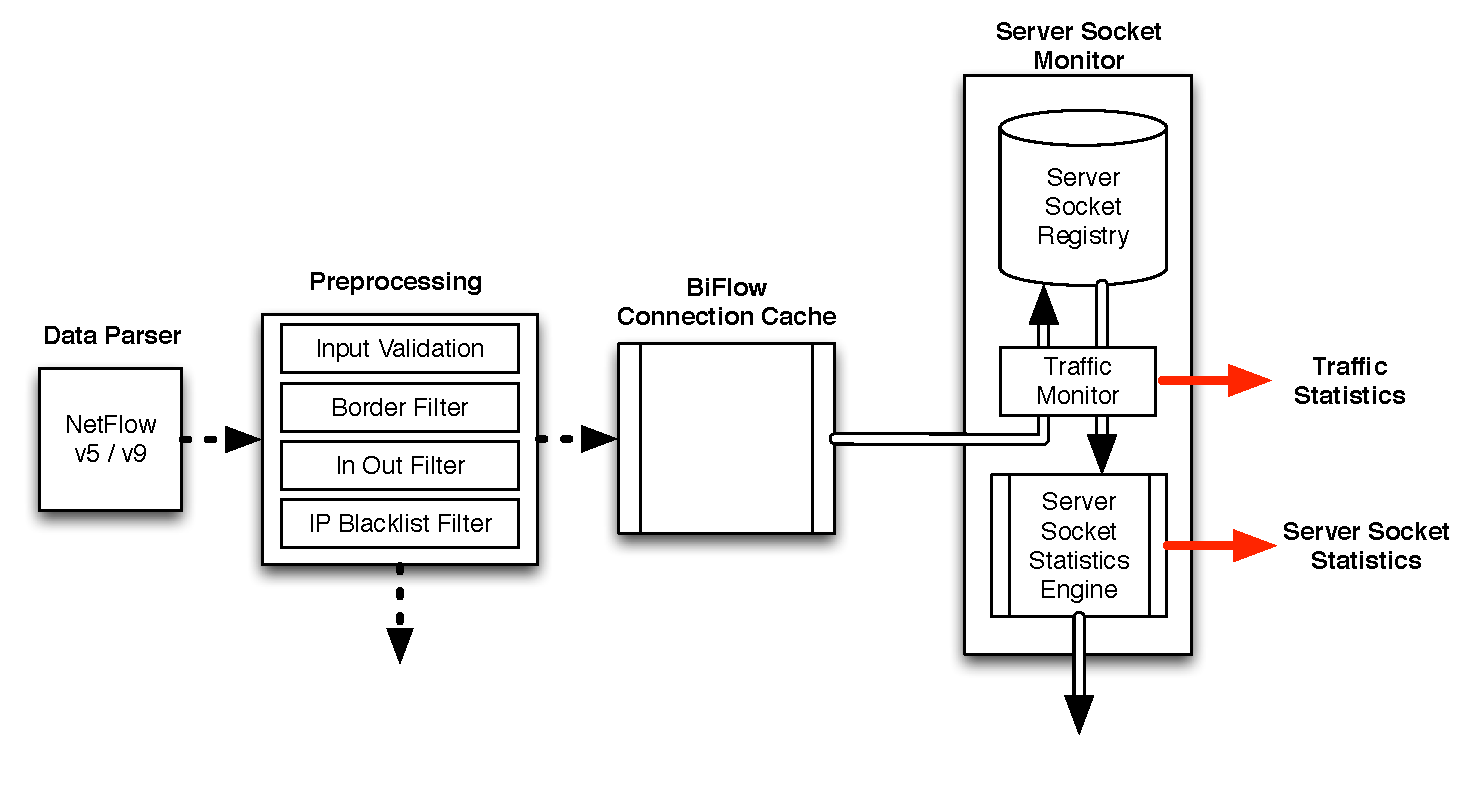
\includegraphics[width=\linewidth]{images/TrackingChain.eps}
	\caption{Processing chain for the server socket monitoring} 
	\label{fig:monitoring_chain} 
\end{figure}

%%%%%%%%%%%%%%%%%%%%%%%%%%%%%%%%%%%%%%%%%%%%%%%%%%%%%%%%%%%%%%%%%%%%%%%%%%%%%%%%
% CHARACTERIZATION SERVERSOCKETS
%%%%%%%%%%%%%%%%%%%%%%%%%%%%%%%%%%%%%%%%%%%%%%%%%%%%%%%%%%%%%%%%%%%%%%%%%%%%%%%%
\newpage
\section{Characterization of Server Sockets 
\label{section:characterization}} The main interest of this thesis is to characterize \emph{server sockets} by its \textbf{stability}, its \textbf{visibility} and its \textbf{popularity}. These properties tries to address the following characteristics of a server socket:

\vbox{ 
\begin{itemize}
	\item \textbf{Stability:} How stable is the \emph{server socket} regarding its responsiveness or availability: 
	\item \textbf{Visibility:} How frequently is the \emph{server socket} contacted by other socket: 
	\item \textbf{Popularity:} How many distinct sockets are contacting the \emph{server socket}: 
\end{itemize}
}

These three characteristics are directly deducible from the statistics observed by the passive monitoring technique outlined in \ref{section:socket_tracking}. In the following, each of the three characteristics are briefly discussed.

\subsection{Stability of a Server Socket} Because of the definition and its detection approach a \emph{server socket} is offering a bidirectional service which means that the client and the \emph{server socket} are both sending packets. Usually, a client socket is opening the connection to a \emph{server socket} which will reply in return to this request. Generally, this also holds for P2P applications as for example bit torrent. However in this case, there may be two \emph{server sockets} involved in the communication and no client socket. Therefore, a \emph{server socket} -- or the communication of it -- can be characterized as stable if all connections of this \emph{server socket} are \textbf{balanced}. 

%%%%%%%%%%% Balanced Connection DEFINITION 	%%%%%%%%%%%%%%%%%%%%%%
\parbox{ 
\textwidth}{ 
\begin{defn}
	{\textbf{Balanced Connection}\\} A connection between two sockets is balanced, if there is one flow originating from each socket which is destined for the other socket. Hence, the connection is bidirectional. 
\end{defn}
}

Thus, the overall stability \emph{server socket} or availability of its service can be approximated by the ratio of the balanced to all connections destined to this \emph{server socket}, i.e. the balanced and the unbalanced. This ratio is referred as a \emph{server socket} \textbf{stability ratio} and is mathematically defined by equation \ref{eq:ratio}. 
\begin{equation}
	\text{Stability}(\text{Socket}_i) = \frac{\text{balanced connections}(\text{Socket}_i)}{\text{balanced connections}(\text{Socket}_i) + \text{unbalanced connections}_{in}(\text{Socket}_i)} 
	\label{eq:ratio} 
\end{equation}

Hence, a \emph{server socket} with a stability ratio of 1 does only have bidirectional connections and thus, replies to all connection attempts. On the other side, a stability ratio of 0 indicates that there are only connections attempts by client sockets, but the server socket never replied upon these request. Unbalanced outgoing connections from the server sockets are indicating a client error or scanning activities of clients with spoofed (internal) source address which are not observed by the monitoring system. Therefore, these unbalanced outgoing connections are not considered for determining the stability ratio at all.

\subsection{Visibility of a Server Socket\label{subsection:visibility}}

% discrete time slots activities of a socket, per day, per 5min slot?
% distribution is heavy-tailed, alot of sockets only rarely connected => due to scanning? due to malware?
The monitoring process of the server sockets is done passively, thus if a server socket is visible in the flow level data of a certain time period, the server socket is active during at that time. Hence, the visibility of a server socket during a certain time interval $t+\Delta{t}$ is a binary measure, either inactive in case it is not visible or active in case it is visible in the data set. Equation \ref{eq:visibility} defines the visibility of a socket during the time interval $t+\Delta{t}$: 
\begin{equation}
	\text{Visibility}_t(\text{Socket}_i,t+\Delta{t}) = \left\{ 
	\begin{array}{l l}
		1 & \quad \text{if $\text{Socket}_i$ is active during $t+\Delta{t}$}\\
		0 & \quad \text{if $\text{Socket}_i$ is not active during $t+\Delta{t}$}\\
	\end{array}
	\right. 
	\label{eq:visibility} 
\end{equation}

In consequence, there are different granularities $\Delta{t}$ to define the visibility a server socket. On the one hand, the most fine-grained resolution is just the flow-level data observation period. In most of the cases, this flow-level data observation period is set to 300 seconds. This fine-grained resolution is referred as the \emph{time slot} resolution, since the entire processing is based on such discrete time slotted data, containing all flows active during this time period. 
On the other hand, there are several other more coarse-grained resolutions of the visibility possible. The most obvious is a day long resolution, i.e. $\Delta{t} = 86400$s.

Furthermore, the visibility of a server socket can be extended from a single time period to the overall observation time, i.e. a week long trace, by summing up the individual visibilities of each time slot as shown in equation \ref{eq:visibility_sum}.
\begin{equation}
	\text{Visibility}(\text{Socket}_i) = \sum_{t} \text{Visibility}_t(\text{Socket}_i,t+\Delta{t})
	\label{eq:visibility_sum} 
\end{equation}

However, this summing approach exacerbate the comparison between different observations since it represents the visibility in absolute terms. Therefore, an even better metric for the visibility of a server socket is to average the individual $\text{Visibility}_t(\text{Socket}_i,t+\Delta{t})$ as outlined by equation \ref{eq:visibility_avg}. This normalizes the visibility to a value in the range between 0 and 1, representing the ratio of its visibility to the maximum visibility possible. Thus, a value of 1 means that the socket is visible in every single time slot and a value of 0 that the socket was never active. 
\begin{equation}
	\overline{\text{Visibility}}(\text{Socket}_i) = \frac{\sum_{t} \text{Visibility}_t(\text{Socket}_i,t+\Delta{t})}{\sum_{t}1}
	\label{eq:visibility_avg} 
\end{equation}

\subsection{Popularity of a Server Socket}

% number of flows / clients?.. degree of Server Socket
Besides the visibility of a server socket, its popularity is another major key characteristics. Whereas the visibility of a server socket defines how frequent in time a socket is contacted by at least one connection endpoint, the popularity of a server socket is defined by the number of connection attempts of client sockets during a certain period of time. The popularity of server socket can be deduced by various metrics as the number of flows, bytes or clients.


%%%%%%%%%%%%%%%%%%%%%%%%%%%%%%%%%%%%%%%%%%%%%%%%%%%%%%%%%%%%%%%%%%%%%%%%%%%%%%%%
% ANALYSIS of SERVER SOCKETS IN THE WILD
%%%%%%%%%%%%%%%%%%%%%%%%%%%%%%%%%%%%%%%%%%%%%%%%%%%%%%%%%%%%%%%%%%%%%%%%%%%%%%%%\newpage
\section{Analysis of Server Sockets in the Wild}

This section covers a detailed analysis of server socket found during a week long data trace from 2010/11/01 00:00:00 UTC until 2010/11/06 00:49:00 UTC, thus covering mainly the first 5 working days in November 2010.

\subsection{Detected Server Sockets}

% sum up of detection parameters > 2 biflows per 5min interval with more TCP 
% packets > 3 UDP > 1
For detecting the server sockets in this observation period, the previously 
discussed detection approach was applied as illustrated by figure 
\ref{fig:detection_chain}. In detail, the connection cache was configured to 
summarize all related unidirectional flow records into a single bidirectional 
flow record during an aggregation interval of 600s. 

After this caching step, these bidirectional flows are filtered by a fan out 
filter implementing the idea of \citet{Allman:2007} to mitigate the effects of 
scanning and p2p churn. This fan out filter is configured to require at least 4 
unidirectional connections with a certain host as source and at least 2 times 
more unidirectional connections than bidirectional connections for classifying 
this host as a scanning host. Previous 
work\citep{Schatzmann:Mining,Schatzmann:Dissection, Schatzmann:Tracing} has 
shown that these parameters are a good choice for efficiently mitigating the 
scanning noise by reducing the scanning spikes of the total traffic volume. 

Moreover, the noise filter is configured to filter all TCP flows with less than 
3 packets in a single direction and UDP flows with less than 1 packet in a 
single direction. 

Furthermore, the server socket detector is configured to extract sockets with a 
degree of 2 or higher as concentrators, thus defining requiring two independent 
connections to a server sockets within 600 seconds. 

% state overall number of detected external and internal server sockets during 
% this period
During the entire observation period of 120.8 hours, the server socket detector 
managed to detect 1'862'389 external server sockets and 609'670 internal server 
sockets.

\subsection{Gravitational Forces of Server Sockets}
% traffic statistics of server sockets detected by type and ratio of traffic 
% towards server sockets
In the following, the overall traffic statistics of the detected server sockets 
are briefly discussed. Figure \ref{fig:flows_by_type} shows the absolute number 
of flows during the entire observation period separated by the type of 
connection. If the flow is destined to a server socket, the flow is denoted as 
monitored, otherwise if as unmonitored. Furthermore, the type of connection also 
considers the balance or direction of the connection, i.e. if the flow is 
bidirectional, unidirectional outgoing or unidirectional incoming. Hence, in 
total there are 6 possible combinations for the type of connection, allowing a 
good interpretation of the detection approach. For easier comparison of each 
type of connection, figure \ref{fig:monitored_flows_by_type} shows the ratio of 
monitored and unmonitored flows by the direction.

In figures \ref{fig:flows_by_type} and \ref{fig:monitored_flows_by_type}, there are two gaps visible around 2010/11/01 10:00 UTC and 2010/11/04 06:05 UTC. These gaps result from missing flow records due to router reboots, collector outages, and storage failures\citep{Schatzmann:Mining}.

\begin{figure}
	[ht] \centering 
	\includegraphics[width=\linewidth]{images/Flows_by_type_area_all_SeS.pdf}
	\caption{Number of flows over time by the type of connection with all detected server sockets} 
	\label{fig:flows_by_type} 
\end{figure}

\begin{figure}[h]
	\centering 
	\includegraphics[width=\linewidth]{images/Flows_monitor_ratio_by_type_all_SeS.pdf}
	\caption{Flows towards known server sockets by traffic type with all detected server sockets} 
	\label{fig:monitored_flows_by_type} 
\end{figure}

Clearly, the dominating kind of the flows are the bidirectional monitored flows 
represented by the red area in figure \ref{fig:flows_by_type}. Comparing this 
share with the bidirectional unmonitored flows represented by the yellow area 
between the red and the green area, yields that the detection approach detects a 
majority of the server sockets. This finding is even better visible on the 
bidirectional ratio of figure \ref{fig:monitored_flows_by_type}. Depending on 
the time of the day, the monitoring ratio of the bidirectional flows is mainly 
between 90\% and 97\%. There are always smaller monitoring ratios during night 
yielding that at night there is a higher share of unknown server sockets active 
than during day. A possible reason for pattern is that there are some server 
sockets which are regularly contacted, however only by very few clients so that 
these sockets get never more than one connection within 600 seconds. Thus, these 
sockets are never detected as concentrators. 

Similarly, if the unidirectional outgoing flows are examined by looking at figure \ref{fig:monitored_flows_by_type}, the monitored flows have predominantly a high share of around 80\% to 90\% of all unidirectional outgoing flows. Figure \ref{fig:flows_by_type} also reveals some high peaks which are probably scanning or backscatter effects which are well visible at November 03 in the night and in the afternoon by the green spikes. However, these green peaks are categorized as monitored unidirectional outgoing flows, thus they must involve at least one known server socket either located external or internal.

Finally, the unidirectional incoming flows have are predominately unmonitored with around 80-97\% of unmonitored flows as it can be seen in figure \ref{fig:monitored_flows_by_type}. Contrasting the trend of the other two categories of traffic, the main reason for this contrast may be that the main part of this unidirectional incoming traffic consists of Internet background radiation \citep{Wustrow10,Pang04} as for example malware scanning. Nevertheless, this unidirectional incoming flow traffic is unimportant with respect to the scope of this thesis.

In a metaphorical sense, server sockets are comparable to masses in physics which are exerting gravitational forces to other objects. Server sockets tend to attract a majority of the observed connections and thus, they are well suitable to represent a majority of the legitimate traffic which is interesting for tracking the end-to-end connectivity.

\todo{Comparing with Port80 SES?!}

\newpage
\subsection{Characterization of Detected Server Sockets}

As discussed in section \ref{section:characterization}, this thesis proposes to characterize server sockets according to their visibility, popularity and stability by different metrics. This section aims to deduce some statistical properties of the detected server sockets regarding these characteristics.

\subsubsection{General Visibility of Server Sockets}

According to \ref{subsection:visibility}, for defining a metric of the visibility of server sockets it is required to define the granularity of a observation period. For reasons of simplicity, two different granularities are defined. One the one hand, a day long observation period yields the number of visible days for the activity of a socket. On the other hand, an observation period of 5 minutes is chosen, since it reflects the default processing interval of FlowBox, allowing a very fine-grained, detailed resolution of a server sockets activity. This second visibility metric is referred as \emph{visible time slots(VTS)}.

\begin{figure}
	[hb] \centering 
	\includegraphics[width=\linewidth]{images/VTS_by_visibledays.pdf}
	\caption{VTS by visible days} 
	\label{fig:vts_by_visibledays} 
\end{figure}

Figure \ref{fig:vts_by_visibledays} shows the number of sockets by the visible time slots separated the number of visible days. The skewness of the 
distributions for 1 to 4 visible days are is very similar. It is obvious that 
the a socket which is visible for only one day cannot exceed 288 visible time 
slot. Nonetheless, considering this daily scaling factor, the distributions are 
looking very similar. Furthermore, figure \ref{fig:vts_by_visibledays} shows 
that the most sockets in absolute terms are only active during one day and only 
in very few visible time slots. 

However, the distribution of the number of sockets with a visibility of 5 or 
even 6 days are slightly different, since there is a higher share of sockets 
with a relatively higher visible time slots, besides the normal scaling factor 
of the number of visible days.

\subsubsection{Visibility and Stability}
Eventually, for selecting those server sockets which are stable and often visible it is of importance to assess the how server sockets are distributed with respect to their stability and visibility characteristic. Hence, figure \ref{fig:rankedVisibility} shows the location of each socket in the field of the ranked visibility and the stability. The ranked visibility is simply defined by the cumulative distribution function of the visibility. Thus, a socket with a ranked visibility of 80\% indicates that there are 80\% of all sockets with the same or lower visibility than this specific socket. 

As figure \ref{fig:rankedVisibility} indicates, the sockets cluster around the top right corner, hence the top visible sockets tend to have a good stability as well.

\begin{figure}
	[hb] \centering 
	\includegraphics[width=\linewidth]{images/visibiliy_stability_map.pdf}
	\caption{Sockets by their ranked visibility and their stability} 
	\label{fig:rankedVisibility} 
\end{figure}


Furthermore, figures \ref{fig:ccdf_ratio_days} and \ref{fig:ccdf_ratio_vts} show 
each a complementary cumulated distribution function of the stability of server 
sockets with different visibilities. 

One the one side, figure \ref{fig:ccdf_ratio_days} is using the daily visibility 
of the sockets. The red curve represents the distribution of the sockets which 
are seen only in one day. Not surprisingly, these group of server sockets reveal 
the highest share of sockets with a stability of 1. This is mainly due to the 
fact that there is a relative high number of server sockets with which are 
active only during a relatively short period of time. This can be justified by 
looking at figure \ref{fig:vts_by_visibledays}.



\begin{landscape}
\begin{figure}
	[p] \centering 
	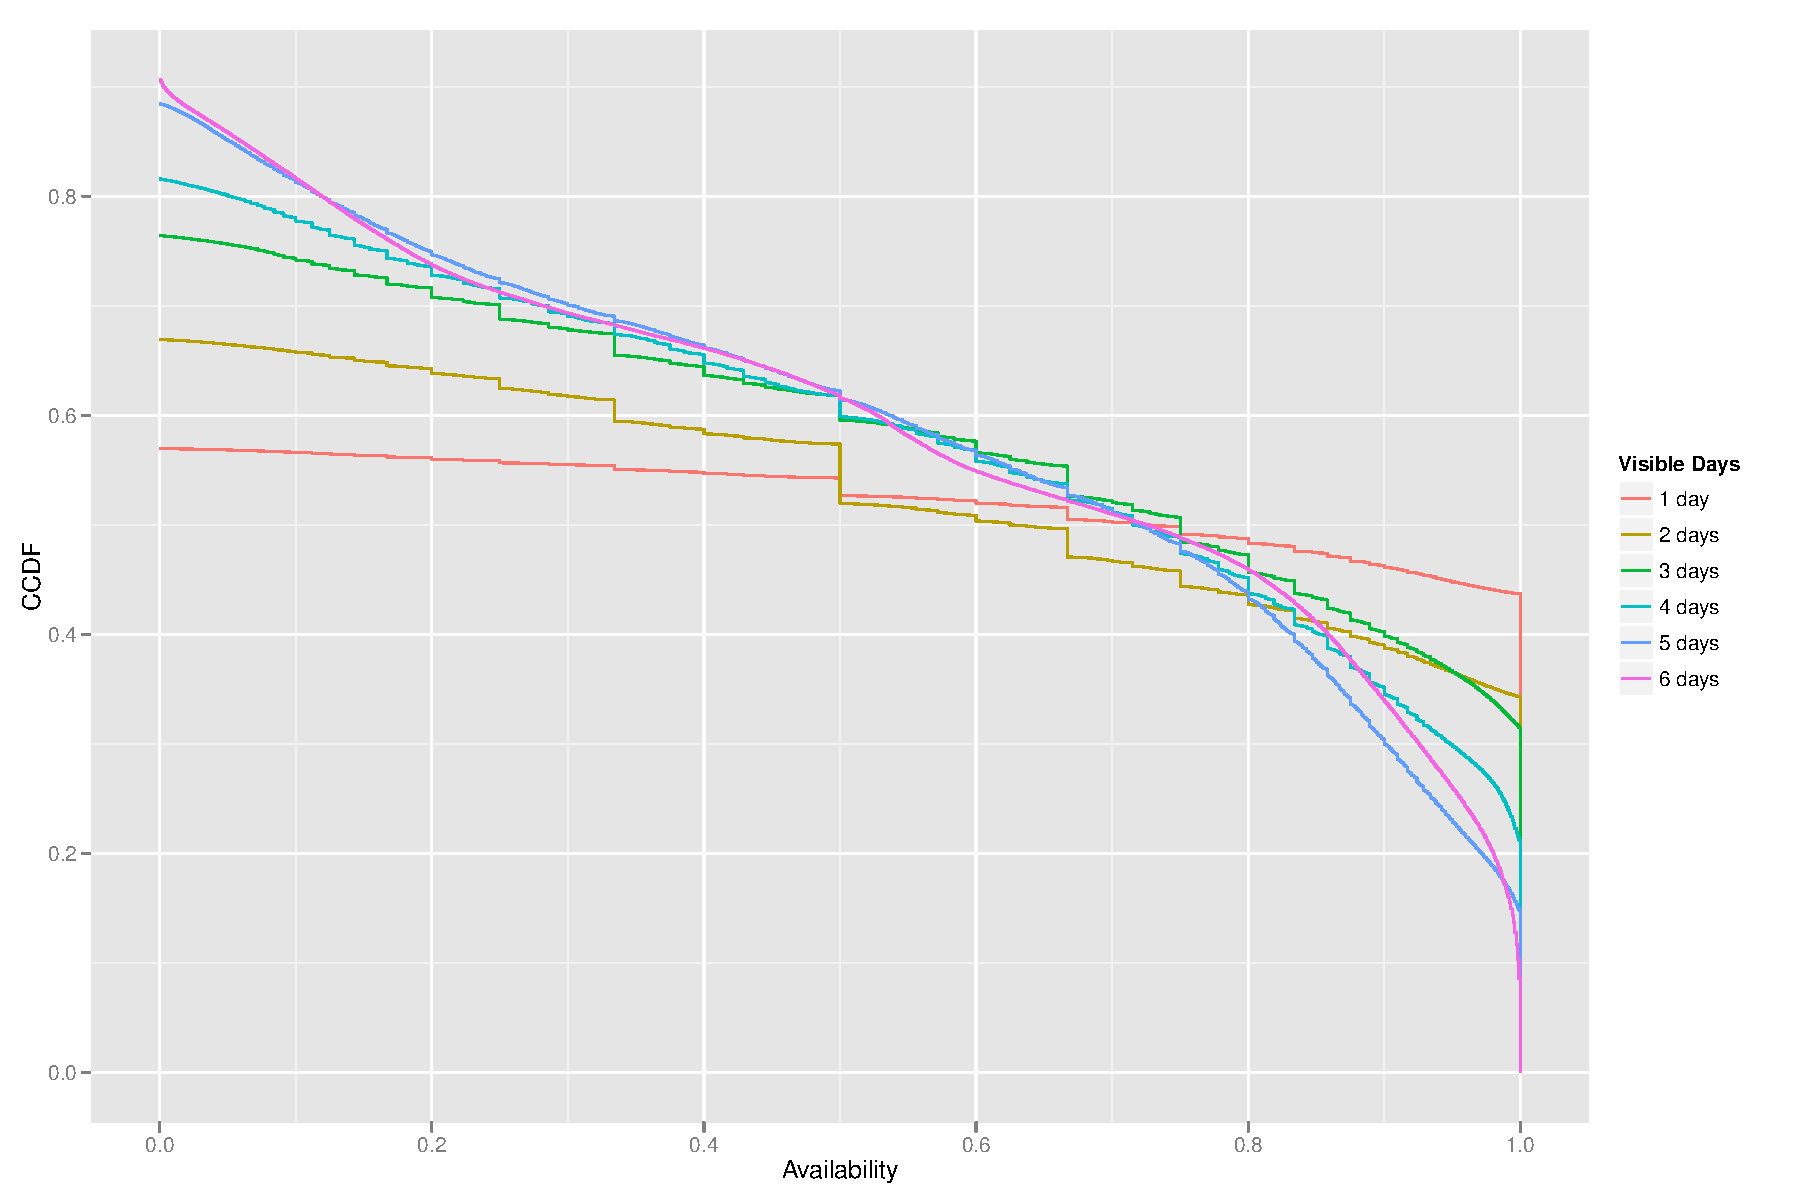
\includegraphics[width=\linewidth]{images/CCDF_ratio_days.pdf}
	\caption{CCDF of the availability by visible days} 
	\label{fig:ccdf_ratio_days} 
\end{figure}
\end{landscape}

\begin{landscape}
\begin{figure}
	[p] \centering 
	\includegraphics[width=\linewidth]{images/CCDF_ratio_VTS.pdf}
	\caption{CCDF of the availability by visible time slots} 
	\label{fig:ccdf_ratio_vts} 
\end{figure}
\end{landscape}

\subsubsection{Popularity and Stability}
Similarly to the visibility, the server sockets characteristics of popularity 
and stability are briefly assessed in the following. The ranked popularity is 
defined in the same way as the ranked visibility. To be precise, the ranked 
popularity is defined as the cumulative distribution function of the popularity 
in terms of flows. Hence, a server socket with a ranked popularity of 80\% 
signifies that there are 80\% of all server socket with a lower or equal 
popularity as this specific socket.


\begin{figure}
	[ht] \centering 
	\includegraphics[width=\linewidth]{images/popularity_stability_map.pdf}
	\caption{Sockets by their ranked popularity and their stability} 
	\label{fig:rankedPopularity} 
\end{figure}


\begin{landscape}
	\begin{figure}
	[p] \centering 
	\includegraphics[width=\linewidth]{images/top20_ratio_box.pdf}
	\caption{Boxer plot of the availability / stability of the top 20 traffic port server sockets} 
	\label{fig:top20_ratio_box} 
\end{figure}
\end{landscape}

\begin{landscape}
\begin{figure}
	[p] \centering 
	\includegraphics[width=\linewidth]{images/top20_visibility_box.pdf}
	\caption{Boxer plot of visibility in days of the top 20 traffic port server sockets}
	\label{fig:top20_visibledays_box}
\end{figure}
\end{landscape}


\begin{table}
	[ht] \centering 
	\begin{tabular}
		{|c|r|r|r|r|r|r|} \hline \textbf{Position} & \textbf{Port} & \textbf{Protocol} & \textbf{Flows} &\textbf{ Flows in \%} & \textbf{Sockets} & \textbf{Sockets in \%}\\
		\hline \hline 1 & 53 & 17 &793851107 & 47.272216 & 314253 & 18.68397\\
		\hline 2 & 80 & 6 &623910956 & 37.152626 & 546735 & 32.50623\\
		\hline 3 & 443 & 6 & 74333936 & 4.426434 & 59800 & 3.555420\\
		\hline 4 & 22 & 6 & 10580812 & 0.630066 & 40363 & 2.399790\\
		\hline 5 & 2703 & 6 & 10139578 & 0.603791 & 22 & 0.001308\\
		\hline 6 & 25 & 6 & 6943533 & 0.413473 & 18560 & 1.103488\\
		\hline 7 & 123 & 17 & 4988781 & 0.297072 & 286 & 0.017004\\
		\hline 8 & 993 & 6 & 3844043 & 0.228905 & 1398 & 0.083118\\
		\hline 9 & 555 & 6 & 3290709 & 0.195955 & 9 & 0.000535\\
		\hline 10 & 995 & 6 & 2411245 & 0.143585 & 654 & 0.038884\\
		\hline 11 & 110 & 6 & 1816240 & 0.108153 & 1211 & 0.072000\\
		\hline 12 & 3789 & 6 & 1796224 & 0.106961 & 10 & 0.000595\\
		\hline 13 & 53 & 6 & 1726716 & 0.102822 & 1102 & 0.065520\\
		\hline 14 & 2128 & 6 & 1677027 & 0.099864 & 390 & 0.023188\\
		\hline 15 & 3478 & 17 & 1607132 & 0.095701 & 176 & 0.010464\\
		\hline 16 & 8080 & 6 & 1362615 & 0.081141 & 2056 & 0.122240\\
		\hline 17 & 3128 & 6 & 1298424 & 0.077319 & 191 & 0.011356\\
		\hline 18 & 5354 & 6 & 1221109 & 0.072715 & 3 & 0.000178\\
		\hline 19 & 8001 & 6 & 1014631 & 0.060419 & 58 & 0.003448\\
		\hline 20 & 21 & 6 & 1010771 & 0.060189 & 1419 & 0.084367\\
		\hline 21 & high & 6 & 37679906 & 2.243762 & 599314 & 35.63233\\
		\hline 22 & high & 17 & 89558306 & 5.333015 & 89820 & 5.340265\\
		\hline 23 & low & 6 & 2505504 & 0.149198 & 3807 & 0.226346\\
		\hline 24 & low & 17 & 749276 & 0.044618 & 302 & 0.017955\\
		\hline 
	\end{tabular}
	\caption{Top 20 port / protocol aggregated sockets by number flows}
	\label{tab:top20_ports}
\end{table}\todo{do something with me..}
SSH TCP 22: Scanning / PW guessing, e.g. X.X.X.X, 6, 22, 1.0, 2, 1, 69.0, 0.0, 0.0 always with 69 or 68 biflows (parallelized? recurring?) $\rightarrow$ that's way such a bad visibility! one-time shots.. /8 network is scanned! meist 3-4 timeslots und nur visibility einem Tag! \ref{tab:top20_ports}\todo{do something with me..}
 

mDNS (5354) $\rightarrow$ Apple mdns resolving; mainly one socket causing this traffic pm-members.apple.com